The European Organization for Nuclear Research (CERN\footnote{The name CERN is derived from the acronym for the French Conseil Europ\'{e}en pour la Recherch Nucl\'{e}aire}) was founded in 1954 and is based in the suburb of Geneva on the Franco\textendash Swiss border.
The main function of CERN is to provide particle accelerators and detectors for high-energy physics research.
The physicists and engineers at CERN are probing the fundamental structure of the universe using the world's largest and most complex scientific facility \textemdash \ the Large Hadron Collider (LHC)~\cite{1748-0221-3-08-S08001}.
In the LHC, the particles are boosted to high energies and collide at close to the speed of light.
The results of the collisions are recorded by the various detectors.
There are seven experiments at the LHC.
The biggest of these experiments are ATLAS (A Toroidal LHC ApparatuS)~\cite{1748-0221-3-08-S08003} and CMS (Compact Muon Solenoid)~\cite{1748-0221-3-08-S08004} which use general-purpose detectors to investigate a broad physics programme ranging from the search for the Higgs boson to extra dimensions and particles that could make up dark matter.
The ALICE (A Large Ion Collider Experiment)~\cite{1748-0221-3-08-S08002} experiment is designed to study the physics of quark-gluon plasma form and the LHCb (Large Hadron Collider beauty)~\cite{1748-0221-3-08-S08005} experiment specializes in investigating of CP violation by studying the $b$-quark.
These four detectors sit underground in huge caverns of the LHC ring.
The rest three experiments, TOTEM~\cite{1748-0221-3-08-S08007}, LHCf~\cite{1748-0221-3-08-S08006}, and MoEDAL~\cite{Pinfold:1181486}, are smaller.
The TOTEM (TOTal Elastic and diffractive cross section Measurement)~\cite{1748-0221-3-08-S08007} experiment aims at the measurement of total cross section, elastic scattering, and diffractive dissociation.
The LHCf (Large Hadron Collider forward)~\cite{1748-0221-3-08-S08006} experiment is intended to measure the neutral particle produced by the collider using the forward particles.
The prime motivation of the MoEDAL (Monopole and Exotics Detector at the LHC)~\cite{Pinfold:1181486} experiment is to search directly for the magnetic monopole.

\section{The Large Hadron Collide}
The LHC~\cite{1748-0221-3-08-S08001} is the world's largest and most powerful accelerator which accelerates and collides protons in a 26.7 km circumference crossing the Franco\textendash Swiss border 100 m underground.
Built in the tunnel of the former LEP (Large Electron\textendash Positron), the LHC is capable of colliding protons as well as heavy ions.
Comparing with the LEP which collides electrons and positrons, the advantage of the LHC is the lower energy loss \footnote{The energy loss for protons is about eleven orders of magnitude smaller than the electrons} in the synchrotron radiation, such that higher energies can be reached by the LHC.
The LHC is designed for collisions at a centre-of-mass energy $\sqrt{s}=14$ TeV and an instantaneous luminosity of $\mathcal{L} =10^{34} \ \textrm{cm}^{-2}\textrm{s}^{-1}$.
Figure~\ref{fig:CERN_accelerator_complex} shows the infrastructure of the LHC and the pre-accelerator system.

\begin{figure}[htbp]
\begin{center}
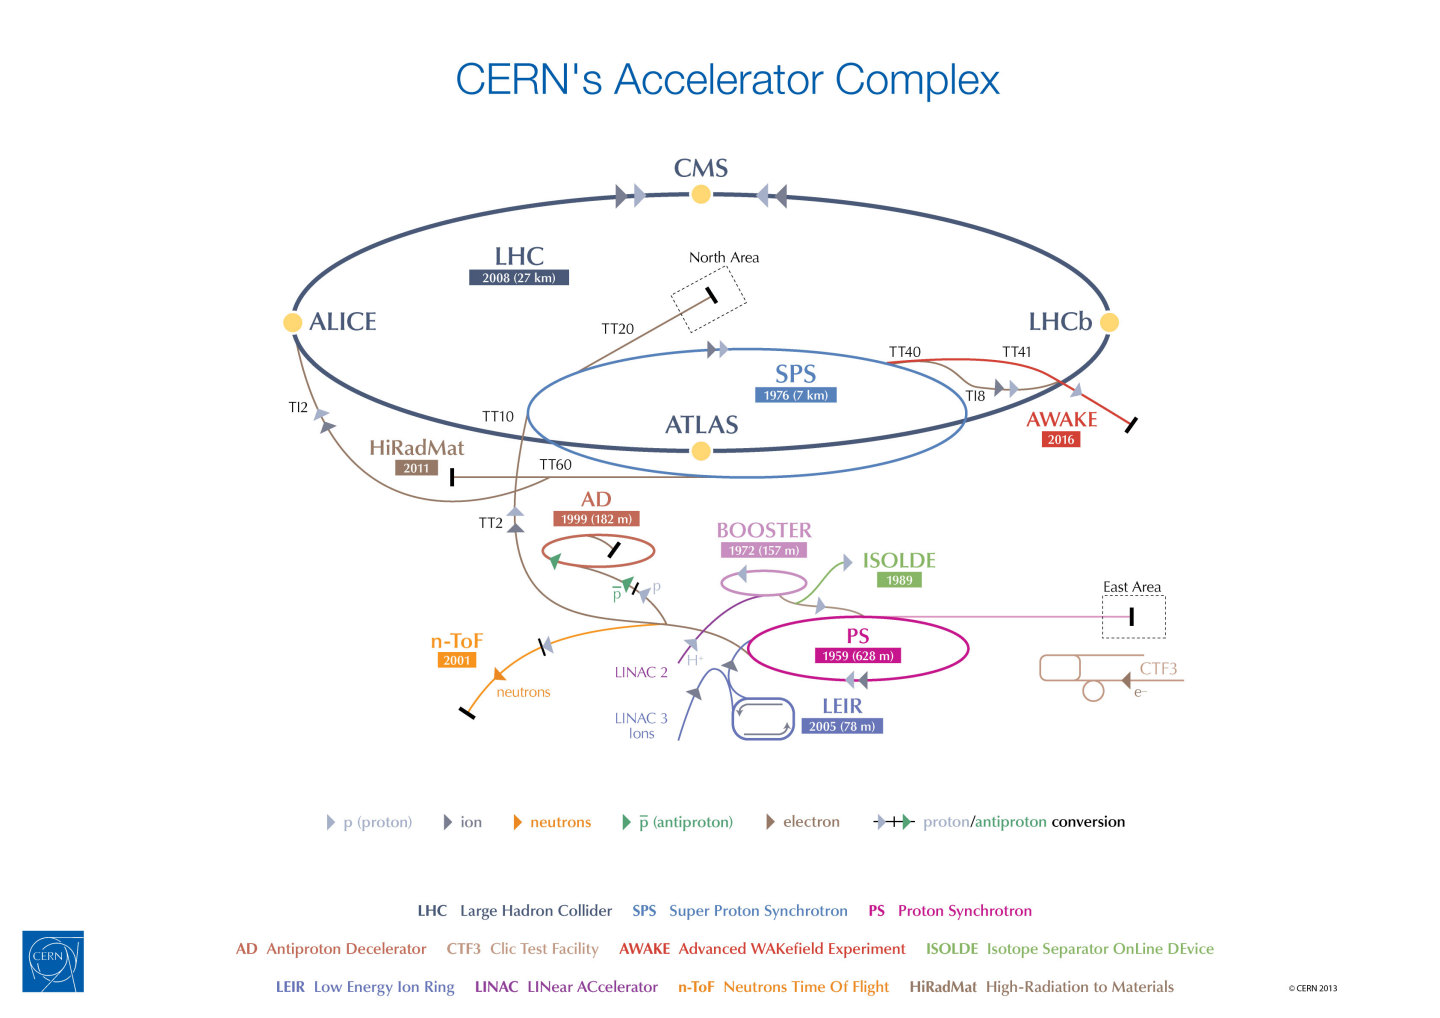
\includegraphics[scale=0.5]{CERN's-accelerator-complex2013.jpg}
\caption{The accelerator complex at CERN~\cite{Marcastel:1621583}.}
\label{fig:CERN_accelerator_complex}
\end{center}
\end{figure}

The protons are extracted by ionization from a hydrogen source and are accelerated to 50 MeV by the linear accelerator LINAC2.
Then they are injected into the Proton Synchrotron Booster (PSB) where the proton energies are increased to 1.4 GeV before they enter the Proton Synchrotron (PS) which accelerates the protons to 25 GeV.
Next, the proton energies are increasing to 450 GeV in the Super Proton Synchrotron (SPS). 
Finally, the protons are split into two beams and enter the LHC where the two beams run in two adjacent beam pipes with opposite directions.
In order to keep the protons on the circular trajectory in the LHC, 1232 superconducting dipole magnets~\cite{1288863} generate a magnetic field strength of 8.33 T to bend the proton beams in eight arcs.
Additionally, 392 quadrupole magnets~\cite{1288863} are installed to focus the beam.
A cryogenic system running with super-fluid helium-4 is used to cool down the superconducting magnets to a temperature of 1.7 K.

For a given physics process, the event rate is proportional to the cross section $\sigma$ of this process.
\begin{equation}
\frac{dN}{dt} = \mathcal{L}\cdot\sigma
\end{equation}
where $N$ is the number of events and $\mathcal{L}$ denotes the luminosity of the beam.
The luminosity of the beam, $\mathcal{L}$ can be calculated by
\begin{equation}
\mathcal{L} = \frac{N^{2} f}{4 \pi \sigma_{x} \sigma_{y}} \cdot F
\end{equation}
where $N$ is the number of protons, $f$ is the bunches crossing frequency, and the $\sigma_{x}$ and $\sigma_{y}$ are the $x$ and $y$ components for cross section $\sigma$.
The geometric luminosity reduction factor, $F$, is related to the crossing angle at the Interaction Point (IP).
Considering a beam consisting of $1.15 \times 10^{11}$ protons with bunching spacing of 25 ns, the transversal size of the bunch at Interaction Pointe $16\times 10^{-4}$ cm, and taking the geometric luminosity reduction factor as 1, the design luminosity of $10^{34}$ cm$^{-2}$s$^{-1}$ can be reached.

The first beam was circulated through the collider on the morning of 10 September 2008~\cite{CERN-COURIER-Sep192008}.
However, a magnet quench incident occurred on 19 September 2008 and caused extensive damage to over 50 superconducting magnets, their mountings, and the vacuum pipe.
Most of 2009 was spent on repairs the damage caused by the magnet quench incident and the operations resumed on 20 November of that year.
The first phase of data-taking (Run 1) started at the end of 2009 and the beam energy was increased to a centre-of-mass $\sqrt{s}=7$ TeV in 2011 and $\sqrt{s} = 8$ TeV in 2012.
The total integrated luminosity of 5.46 fb$^{-1}$ was collected in 2011 and of 22.8 fb$^{-1}$ was collected in 2012.
Since 13 February 2013 the LHC was in the Long Shutdown 1 (LS1) phase for maintenance and upgrades.
On 5 April 2015, the LHC restarted and was operating at a centre-of-mass energy $\sqrt{s}=13$ TeV throughout the Run 2 phase\footnote{The Run 2 data-taking started from 2015}.



\section{The ATLAS experiment}

\subsection{The Inner Detector}

\subsection{The Calorimeter}

\subsection{The Muon Spectrometer}

\subsection{The Trigger system}

\subsection{}